\documentclass[tikz]{standalone}
\usepackage{tikz}
\usepackage{graphicx}

\usetikzlibrary{calc, angles, quotes}
\usetikzlibrary{intersections} % Necessário para achar pontos de cruzamento

\begin{document}
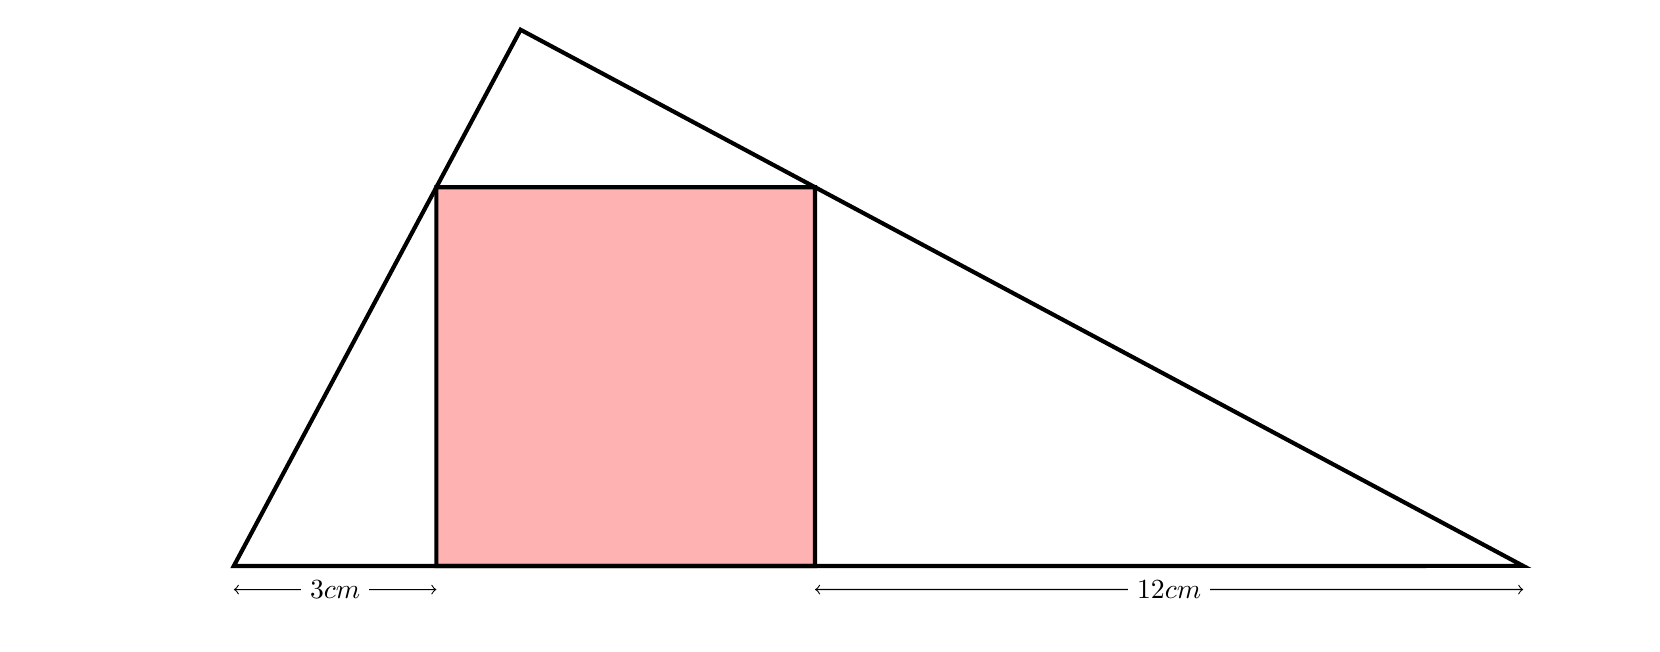
\begin{tikzpicture}[scale=1]
  \coordinate (A) at (-2.69,-1.9);
  \coordinate (B) at (1,5) node[right] {B};

% Paths
  \path[name path=line1] (A) -- (B);
  \path[name path=line2] (B) -- ($(B)!16cm!90:(A)$);
  \path[name path=line3] (-3,3) -- (5,3);
  \path [red, opacity=0.5, name intersections={of=line1 and line3}]
    (intersection-1) coordinate (p1); 
  \path [red, opacity=0.5, name intersections={of=line2 and line3}]
    (intersection-1) coordinate (p2); 

% Quadrado
  \draw[line width=1.5pt,fill=red!30] (p1) -- (p2) -- ($(p2)!1!90:(p1)$) coordinate (p3) 
                          -- ($(p3)!1!90:(p2)$) coordinate (p4)
                          -- cycle;
%Paths de base (angle1)
  \path[name path=line4] ($(p3)!10cm!(p4)$) -- (p4) -- ($(p4)!15cm!(p3)$); 
  
  \path [red, opacity=0.5, name intersections={of=line1 and line4}]
    (intersection-1) coordinate (angle1);
  \path [red, opacity=0.5, name intersections={of=line2 and line4}]
    (intersection-1) coordinate (angle2);

% Triângulo
  \draw[line width=1.5pt] (angle1) -- (B) -- (angle2) -- cycle;
  
  \draw[<->] ([yshift=-3mm]angle1) -- ([yshift=-3mm]p4) node[midway,fill=white] {$3cm$};
  \draw[<->] ([yshift=-3mm]angle2) -- ([yshift=-3mm]p3) node[midway,fill=white] {$12cm$};
\end{tikzpicture}


\end{document}